\chapter{Schaltkreisentwurf}

\section{Abstraktionsebenen und Sichten}
	\paragraph{Ebenen des Entwurfs:}
	\begin{itemize}
		\item Charakterisierung des jeweiligen Detailiertheitsgrades der Beschreibung des Entwurfsgrades
		\item Abstraktionsgrad von der eigentlichen physikalischen Realisierung
		\item Abstraktionsniveaus, Hierarchien
	\end{itemize}

	\paragraph{Sichten des Entwurfs:}
	\begin{itemize}
		\item Betrachtung des Entwurfsgegenstandes aus verschiedenen Richtungen
		\item Sicht = Eigenschaften die den Entwurfsgegenstand Charakterisieren
		\item Alle Sichten auf jeder Entwurfseben $\Rightarrow$ Y-Diagramm / x-Diagramm
	\end{itemize}

\subsection{Abstraktionsebenen}
	\paragraph{Systemebene (system level):} Systemkonzept des Entwurfsgegenstandes
	\paragraph{Algorithmische Ebene (algorithm level):} Algorithmische Beschreibung des Entwurfsgegenstandes
	\paragraph{Register-Transfer Ebene (register-transfer-level - RTL):} Datentransfer und -verarbeitung zwischen Registern
	\paragraph{Logikebene (gate level):} Beschreibung auf Gatterniveau
	\paragraph{Schaltkreiseben:} Transistorebene im weiteren Sinne, umfasst:
		\begin{itemize}
			\item Schalterebene
			\item Schaltungsebene
			\item Bauelementebene
			\item Technologieebene
		\end{itemize}

\subsection{Sichten}
	\paragraph{Verhaltenssicht:} Beschreibung des zeitlichen Verhaltens durch charaktersierende Variablen und deren Werteverläufe über die Zeit
		
		\begin{center}
			\boldmath\( \mathlarger{\vec{y}(t) = f(\vec{x}(t))} \)
		\end{center}
	\paragraph{Struktursicht:} Spezifizierung eines Objektes durch Subobjekte und deren Verbindungsstrukturen
	
	\paragraph{Geometriesicht:} Räumliche Ausdehnung der Subobjekte
	
	\paragraph{Testsicht:} Existenz oder Nichtexistenz angenommener struktureller oder funktionaler Defekte \\(F. J. Rammig, Systematischer Entwurf digitaler Systeme, B.G Teubner Stuttgart 1989)
	
\subsection{Y-Diagramm nach Gajski}
	\begin{itemize}
		\item Stellt Ebenen und Sichten in FOrm eines Y-Diagrammes dar
		\item Ursprünglich nur 3 Ebenen
		\item Heute: Erweiterung auf 5 Ebenen:
			\begin{itemize}
				\item Systemebene
				\item Algorithmische Ebene
				\item Register-Transfer Ebene
				\item Logikeben
				\item Schaltkreisebene
			\end{itemize}
	\end{itemize}
	\begin{center}
		\includegraphics[page=9, width=0.8\linewidth, trim=30mm 20mm 20mm 40mm, clip]{\Path/resources/Vorlesung/VLSI/02_Schaltkreisentwurf.pdf}
		\\\includegraphics[page=10, width=0.8\linewidth, trim=30mm 20mm 20mm 40mm, clip]{\Path/resources/Vorlesung/VLSI/02_Schaltkreisentwurf.pdf}
	\end{center}
	
\newpage
\section{Entwurfsablauf}
	\paragraph{Allgemein:} Transformation einer Aufgabenstellung (Pflichtenheft) in einen fertigen Schaltkreis
	\paragraph{Top-Down-Strategie:}
		\begin{itemize}
			\item Systemebene $\rightarrow$ Schaltkreisebene
			\item Vorteil: Parallele Entwicklung auf unteren Ebenen
			\item Nachteil: Systemspezifikation zu Projektbeginn oft zu ungenau
		\end{itemize}
	\paragraph{Bottom-Up-Strategie:}
		\begin{itemize}
			\item Analyse vorhandener Komponenten
			\item Zusammensetzen von neuen Komponenten auf höherer Ebene im Sinne der Aufgabenstellung
			\item Nachteil: globales Ziel wird nicht immer erreicht
		\end{itemize}
	\paragraph{$\Rightarrow$ Meet-in-the-Middle}
	
	\paragraph{Entwurfsschritt:}
		\begin{itemize}
			\item generierende Aktivität
			\item überprüfende Aktivität
		\end{itemize}
	\paragraph{Syntheseschritt:}
		\begin{itemize}
			\item Abbildung eines Entwurfsschrittes in Richtung auf das Entwurfsziel
			\item Abstraktionsgrad sinkt, Detailhiertheitsgrad steigt
			\item Einbringung neuer Informationen
		\end{itemize}
	\paragraph{Analyseschritt:}
		\begin{itemize}
			\item Abbildung eines Entwurfsschrittes in umgekehrter Richtung zum Syntheseschritt
			\item Gewinnung abstrakter Informationen durch Zusammenfassen und Generalisieren von Details (Extraktionsprozess)
			\item Beispiel: Validierung eines Syntheseschrittes
		\end{itemize}
		
	\begin{center}
		\includegraphics[page=13, width=0.39\linewidth, trim=40mm 30mm 40mm 50mm, clip]{\Path/resources/Vorlesung/VLSI/02_Schaltkreisentwurf.pdf}
		\includegraphics[page=14, width=0.6\linewidth, trim=0mm 30mm 0mm 45mm, clip]{\Path/resources/Vorlesung/VLSI/02_Schaltkreisentwurf.pdf}
	\end{center}
	
\newpage
\section{Entwurfsstile}
	\begin{center}
		\includegraphics[page=15, width=0.8\linewidth, trim=40mm 28mm 40mm 60mm, clip]{\Path/resources/Vorlesung/VLSI/02_Schaltkreisentwurf.pdf}
	\end{center}
	
	\subsubsection{Gegenüberstellung Entwurfsalternativen}
		\begin{center}
			\includegraphics[page=16, width=0.8\linewidth, trim=35mm 28mm 30mm 60mm, clip]{\Path/resources/Vorlesung/VLSI/02_Schaltkreisentwurf.pdf}
		\end{center}

\subsection{Full-Custom Entwurf}
	\begin{center}
		\includegraphics[page=17, width=0.8\linewidth, trim=40mm 28mm 40mm 60mm, clip]{\Path/resources/Vorlesung/VLSI/02_Schaltkreisentwurf.pdf}
	\end{center}
	\paragraph{Merkmale:}
	\begin{itemize}
		\item Platzierung und Verdrahtung selbst entworfener Transistoren \& Gatter
		\item Auch Mischung von Analog- und Digitaltechnik, z.B. für spezielle I/O-Signaltreiber
		\item Erfüllung spezieller Anforderungen, z.B. gehärtet gegen Strahlung
		\item Häufig nur auf kleine Teilschaltungen angewendet
		\item Hoch qualifizierte Entwicklungsingenieure mit Detailkenntnissen zu den Prozessen erforderlich
	\end{itemize}
	\paragraph{Anwendung:}
	\begin{itemize}
		\item Sensorik, Mixed-Signal-Schaltungen
		\item Raumfahrt
	\end{itemize}
	\subsubsection{Beispiel: Inverter}
		\begin{center}
			\includegraphics[page=19, width=0.8\linewidth, trim=40mm 28mm 40mm 60mm, clip]{\Path/resources/Vorlesung/VLSI/02_Schaltkreisentwurf.pdf}
		\end{center}
	
\newpage
\subsection{Standardzellenentwurf}
	\begin{center}
		\includegraphics[page=20, width=0.8\linewidth, trim=40mm 28mm 40mm 60mm, clip]{\Path/resources/Vorlesung/VLSI/02_Schaltkreisentwurf.pdf}
	\end{center}
	\paragraph{Merkmale:}
	\begin{itemize}
		\item Platzierung und Verdrahtung vorgegebener Gatter- oder Makrozellen
		\item Auswahl einer Technologiebibliothek nach:
			\begin{itemize}
				\item Fertigungstechnologie, Strukturbreite und Funktion
				\item High-Speed, Low-Leakage oder Mischung aus Beidem
			\end{itemize}
		\item Werkzeuggestützte Platzierung und Verdrahtung
		\item Makrozellen:
			\begin{itemize}
				\item Vordefiniert oder per Generator kundenspezifisch erzeugt
				\item Bsp: RAM, ALU, I/O-Komponenten
			\end{itemize}
	\end{itemize}
	\paragraph{Anwendung:}
	\begin{itemize}
		\item Anwendungsspezifische Schaltkreise mit hohen Stückzahlen
		\item Starke Optimierung bzgl. Chipfläche, Geschwindigkeit und Verlustleistung
	\end{itemize}
	\subsubsection{Konventionelle Architektur vs. Strukturierte Architektur}
		\begin{center}
			\includegraphics[page=22, width=0.45\linewidth, trim=60mm 28mm 60mm 60mm, clip]{\Path/resources/Vorlesung/VLSI/02_Schaltkreisentwurf.pdf}
			\includegraphics[page=23, width=0.45\linewidth, trim=60mm 28mm 60mm 60mm, clip]{\Path/resources/Vorlesung/VLSI/02_Schaltkreisentwurf.pdf}
		\end{center}
	
\newpage
\subsection{Maskenprogrammierbare Gate Arrays}
	\begin{center}
		\includegraphics[page=27, width=0.8\linewidth, trim=40mm 28mm 40mm 60mm, clip]{\Path/resources/Vorlesung/VLSI/02_Schaltkreisentwurf.pdf}
	\end{center}
	\paragraph{Merkmale:}
	\begin{itemize}
		\item Festlegung der Funktion mittels Masken bei der Halbleiterfertigung
		\item Ausgewählte Masken: teilweise vorgefertigte IC (Master)
		\item Beispiele:
			\begin{itemize}
				\item MPGA (Maskprogrammable Gate-Array): auch MGA
					\begin{itemize}
						\item Vorgefertigte universelle Gatter/Makros mit fester Anordnung
						\item Verdrahtung kundenspezifisch
					\end{itemize}
				\item MROM: ROM dessen Inhalt vom Kunden mit Masken festgelegt wird
			\end{itemize}
	\end{itemize}
	\paragraph{Anwendung:}
	\begin{itemize}
		\item Anwendungsspezifische Schaltkreise bei mittleren Stückzahlen
		\item Kostenoptimiert mit reduzierten Optimierungspotential
	\end{itemize}
	\subsubsection{MPGA}
		\begin{center}
			\includegraphics[page=29, width=0.45\linewidth, trim=60mm 28mm 60mm 60mm, clip]{\Path/resources/Vorlesung/VLSI/02_Schaltkreisentwurf.pdf}
		\end{center}
	
	
\newpage
\subsection{Anwenderprogrammierbare IC}
	\begin{center}
		\includegraphics[page=30, width=0.8\linewidth, trim=40mm 28mm 40mm 60mm, clip]{\Path/resources/Vorlesung/VLSI/02_Schaltkreisentwurf.pdf}
	\end{center}
	\paragraph{Merkmale:}
	\begin{itemize}		
		\item Field-Programmable $\Leftrightarrow$ feldprogrammierbar
		\item Vor Ort (im Feld) vom Anwender programmierbar
		\item Hardware ist fix. Funktionalität kann aber mittels spezieller Konfiguration \grqq programmiert\grqq werden
	\end{itemize}
	\paragraph{Anwendung:}
	\begin{itemize}
		\item Anwendungsspezifische IC bei kleinen und mittleren Stückzahlen
		\item Mehrfach neu programmierbar zwecks Optimierung und Fehlerbehebung, auch während des praktischen Einsatzes
		\item Einfache Integration eines ganzen Systems auf einem Chip
		\item Prototyping, HW-/SW-Codesign
	\end{itemize}
	\subsubsection{Hardwareprogrammierung}
		\begin{center}
		\includegraphics[page=21, width=0.7\linewidth, trim=30mm 20mm 20mm 40mm, clip]{\Path/resources/Vorlesung/VLSI/01_Einfuehrung.pdf}
		\end{center}
	\subsubsection{Klassifikation Anwenderprogrammierbare IC}
		\begin{center}
			\includegraphics[page=33, width=0.8\linewidth, trim=35mm 28mm 30mm 58mm, clip]{\Path/resources/Vorlesung/VLSI/02_Schaltkreisentwurf.pdf}
		\end{center}
	\subsubsection{CPLD}
		Globale Vernetzung einer kleiner Anzahl von Funktionsblöcken (FB)
		\begin{center}
			\includegraphics[page=34, width=0.8\linewidth, trim=35mm 23mm 30mm 70mm, clip]{\Path/resources/Vorlesung/VLSI/02_Schaltkreisentwurf.pdf}
		\end{center}
	\subsubsection{CPLD-Funktionsblock}
		Funktionsblock bestehend aus PLA (Und/Oder-Matrix) und Makrozellen (MC)
		\begin{center}
			\includegraphics[page=35, width=0.5\linewidth, trim=35mm 23mm 30mm 70mm, clip]{\Path/resources/Vorlesung/VLSI/02_Schaltkreisentwurf.pdf}
		\end{center}
	\subsubsection{PLA}
		\begin{center}
			\includegraphics[page=36, width=0.8\linewidth, trim=35mm 23mm 30mm 40mm, clip]{\Path/resources/Vorlesung/VLSI/02_Schaltkreisentwurf.pdf}
		\end{center}
	\subsubsection{Makrozellen + I/O-Block}
		Verschiedene Betriebsspannungen für digitale Lokig (Core) und I/O-Pads
		\begin{center}
			\includegraphics[page=37, width=0.8\linewidth, trim=35mm 23mm 30mm 70mm, clip]{\Path/resources/Vorlesung/VLSI/02_Schaltkreisentwurf.pdf}
		\end{center}
		\paragraph{Konfiguration der Makrozelle:}	
		\begin{center}
			\includegraphics[page=38, width=0.8\linewidth, trim=35mm 93mm 30mm 70mm, clip]{\Path/resources/Vorlesung/VLSI/02_Schaltkreisentwurf.pdf}
		\end{center}
		\paragraph{Steuerung des I/O-Blocks:}\hfill\\
		Umschaltung des I/O-Pins zwischen Ein- und Ausgang (Tri-State) zur Laufzeit mittels seperatem Produktterm möglich.
	
	\subsubsection{FPGA-Architektur}	
		\begin{center}
			\includegraphics[page=39, width=0.8\linewidth, trim=35mm 30mm 20mm 58mm, clip]{\Path/resources/Vorlesung/VLSI/02_Schaltkreisentwurf.pdf}
		\end{center}
	
\section{Entwurfswerkzeuge}
	\begin{center}
		\includegraphics[page=40, width=0.8\linewidth, trim=35mm 87mm 30mm 65mm, clip]{\Path/resources/Vorlesung/VLSI/02_Schaltkreisentwurf.pdf}
	\end{center}
	Auswahl CAD-Werkzeuge:
	\begin{itemize}
		\item Cadence
		\item Xilinx ISE
		\item Altera Quartus
		\item Synopsys
	\end{itemize}
	
	
	
	
	
